\documentclass[12pt,twoside]{article}
%%%%%%%%%%%%%%%%%%%%%%%%%%%%%%%%%%%%%%%%%%%%%%%%%%%%%%%%%%%%%
% Meta informations:
\newcommand{\trauthor}{Leena Chennuru Vankdara}
\newcommand{\trtype}{Seminar Paper} %{Seminararbeit} %{Proseminararbeit}
\newcommand{\trcourse}{Biologically Inspired Artificial Intelligence}
\newcommand{\trtitle}{Cortical Computing for Invariant Object Recognition}
\newcommand{\trmatrikelnummer}{6641141}
\newcommand{\tremail}{4chennur@informatik.uni-hamburg.de}
\newcommand{\trarbeitsbereich}{Knowledge Technology, WTM}
\newcommand{\trdate}{25.12.2014}

%%%%%%%%%%%%%%%%%%%%%%%%%%%%%%%%%%%%%%%%%%%%%%%%%%%%%%%%%%%%%
% Languages:

% Falls die Ausarbeitung in Deutsch erfolgt:
% \usepackage[german]{babel}
% \usepackage[T1]{fontenc}
% \usepackage[latin1]{inputenc}
% \usepackage[latin9]{inputenc}	 				
% \selectlanguage{german}

% If the thesis is written in English:
\usepackage[english]{babel} 						
\selectlanguage{english}

%%%%%%%%%%%%%%%%%%%%%%%%%%%%%%%%%%%%%%%%%%%%%%%%%%%%%%%%%%%%%
% Bind packages:
\usepackage{acronym}                    % Acronyms
\usepackage{algorithmic}								% Algorithms and Pseudocode
\usepackage{algorithm}									% Algorithms and Pseudocode
\usepackage{amsfonts}                   % AMS Math Packet (Fonts)
\usepackage{amsmath}                    % AMS Math Packet
\usepackage{amssymb}                    % Additional mathematical symbols
\usepackage{amsthm}
\usepackage{booktabs}                   % Nicer tables
%\usepackage[font=small,labelfont=bf]{caption} % Numbered captions for figures
\usepackage{color}                      % Enables defining of colors via \definecolor
\definecolor{uhhRed}{RGB}{254,0,0}		  % Official Uni Hamburg Red
\definecolor{uhhGrey}{RGB}{122,122,120} % Official Uni Hamburg Grey
\usepackage{fancybox}                   % Gleichungen einrahmen
\usepackage{fancyhdr}										% Packet for nicer headers
%\usepackage{fancyheadings}             % Nicer numbering of headlines

%\usepackage[outer=3.35cm]{geometry} 	  % Type area (size, margins...) !!!Release version
%\usepackage[outer=2.5cm]{geometry} 		% Type area (size, margins...) !!!Print version
%\usepackage{geometry} 									% Type area (size, margins...) !!!Proofread version
\usepackage[outer=3.15cm]{geometry} 	  % Type area (size, margins...) !!!Draft version
\geometry{a4paper,body={5.8in,9in}}

\usepackage{graphicx}                   % Inclusion of graphics
%\usepackage{latexsym}                  % Special symbols
\usepackage{longtable}									% Allow tables over several parges
\usepackage{listings}                   % Nicer source code listings
\usepackage{multicol}										% Content of a table over several columns
\usepackage{multirow}										% Content of a table over several rows
\usepackage{natbib}
\usepackage{rotating}										% Alows to rotate text and objects
\usepackage[hang]{subfigure}            % Allows to use multiple (partial) figures in a fig
%\usepackage[font=footnotesize,labelfont=rm]{subfig}	% Pictures in a floating environment
\usepackage{tabularx}										% Tables with fixed width but variable rows
\usepackage{url,xspace,boxedminipage}   % Accurate display of URLs
\usepackage{wrapfig}

%%%%%%%%%%%%%%%%%%%%%%%%%%%%%%%%%%%%%%%%%%%%%%%%%%%%%%%%%%%%%
% Configurationen:

\hyphenation{whe-ther} 									% Manually use: "\-" in a word: Staats\-ver\-trag

%\lstloadlanguages{C}                   % Set the default language for listings
\DeclareGraphicsExtensions{.pdf,.svg,.jpg,.png,.eps} % first try pdf, then eps, png and jpg
\graphicspath{{./src/}} 								% Path to a folder where all pictures are located
\pagestyle{fancy} 											% Use nicer header and footer

% Redefine the environments for floating objects:
\setcounter{topnumber}{3}
\setcounter{bottomnumber}{2}
\setcounter{totalnumber}{4}
\renewcommand{\topfraction}{0.9} 			  %Standard: 0.7
\renewcommand{\bottomfraction}{0.5}		  %Standard: 0.3
\renewcommand{\textfraction}{0.1}		  	%Standard: 0.2
\renewcommand{\floatpagefraction}{0.8} 	%Standard: 0.5

% Tables with a nicer padding:
\renewcommand{\arraystretch}{1.2}

%%%%%%%%%%%%%%%%%%%%%%%%%%%%
% Additional 'theorem' and 'definition' blocks:
\theoremstyle{plain}
\newtheorem{theorem}{Theorem}[section]
%\newtheorem{theorem}{Satz}[section]		% Wenn in Deutsch geschrieben wird.
\newtheorem{axiom}{Axiom}[section] 	
%\newtheorem{axiom}{Fakt}[chapter]			% Wenn in Deutsch geschrieben wird.
%Usage:%\begin{axiom}[optional description]%Main part%\end{fakt}

\theoremstyle{definition}
\newtheorem{definition}{Definition}[section]

%Additional types of axioms:
\newtheorem{lemma}[axiom]{Lemma}
\newtheorem{observation}[axiom]{Observation}

%Additional types of definitions:
\theoremstyle{remark}
%\newtheorem{remark}[definition]{Bemerkung} % Wenn in Deutsch geschrieben wird.
\newtheorem{remark}[definition]{Remark} 

%%%%%%%%%%%%%%%%%%%%%%%%%%%%
% Provides TODOs within the margin:
\newcommand{\TODO}[1]{\marginpar{\emph{\small{{\bf TODO: } #1}}}}

%%%%%%%%%%%%%%%%%%%%%%%%%%%%
% Abbreviations and mathematical symbols
\newcommand{\modd}{\text{ mod }}
\newcommand{\RS}{\mathbb{R}}
\newcommand{\NS}{\mathbb{N}}
\newcommand{\ZS}{\mathbb{Z}}
\newcommand{\dnormal}{\mathit{N}}
\newcommand{\duniform}{\mathit{U}}

\newcommand{\erdos}{Erd\H{o}s}
\newcommand{\renyi}{-R\'{e}nyi}
%%%%%%%%%%%%%%%%%%%%%%%%%%%%%%%%%%%%%%%%%%%%%%%%%%%%%%%%%%%%%
% Document:
\begin{document}
\renewcommand{\headheight}{14.5pt}

\fancyhead{}
\fancyhead[LE]{ \slshape \trauthor}
\fancyhead[LO]{}
\fancyhead[RE]{}
\fancyhead[RO]{ \slshape \trtitle}

%%%%%%%%%%%%%%%%%%%%%%%%%%%%
% Cover Header:
\begin{titlepage}
	\begin{flushleft}
		Universit\"at Hamburg\\
		Department Informatik\\
		\trarbeitsbereich\\
	\end{flushleft}
	\vspace{3.5cm}
	\begin{center}
		\huge \trtitle\\
	\end{center}
	\vspace{3.5cm}
	\begin{center}
		\normalsize\trtype\\
		[0.2cm]
		\Large\trcourse\\
		[1.5cm]
		\Large \trauthor\\
		[0.2cm]
		\normalsize Matr.Nr. \trmatrikelnummer\\
		[0.2cm]
		\normalsize\tremail\\
		[1.5cm]
		\Large \trdate
	\end{center}
	\vfill
\end{titlepage}

	%backsite of cover sheet is empty!
\thispagestyle{empty}
\hspace{1cm}
\newpage

%%%%%%%%%%%%%%%%%%%%%%%%%%%%
% Abstract:

% Abstract gives a brief summary of the main points of a paper:
\section*{Abstract}
In this paper, we try to provide a bird's eye view of biologically inspired models of visual recognition. The focus of this paper is to identify some of components of the class of biologically inspired visual recognition systems and to identify the optimality of parameters for each of the components and answer some questions that would lead to construction of what we refer to as the optimal biologically inspired hierarchical architecture for object recognition.

% Lists:
\setcounter{tocdepth}{2} 					% depth of the table of contents (for Seminars 2 is recommented)
\tableofcontents
\pagenumbering{arabic}
\clearpage

%%%%%%%%%%%%%%%%%%%%%%%%%%%%
% Content:

% the actual content, usually separated over a number of sections
% each section is assigned a label, in order to be able to put a
% crossreference to it

\section{Introduction}
\label{sec:introduction}
Invariant object recognition and coherent object representation have been major hurdles in developing efficient artificial vision systems. Invariant object recognition forms the core of the problem of developing egocentrical object based representations of the external world. Given the incredible ability of the biological vision systems which exhibit invariance to a considerable amount of deformation, it is natural to take inspiration from biological vision systems to build artificial vision systems capable of performing invariant object recognition. In this paper, we evaluate different hierarchical models which attempt to mimic the cortical circuit design and the cortical architecture found in the neocortex of the brain to achieve object recognition. In the next section, a brief summary of design principles of cortical computing is presented along with a model \cite{Grossberg2007} linking the designs of cortical computing to behavioral properties of various forms of biological intelligence. In the third section, we define the problem of invariance in object recognition\cite{rohtua} and the challenges faced by Artificial Vision systems which try to achieve this goal. In the fourth section, We provide a brief summary of biologically inspired models for invariant object recognition\cite{Fukushim1980}\cite{JimMutch2008}\cite{NicolasPinto2009}\cite{MarkusLessmann2014}\cite{ThomasSerre2007}\cite{XiaolinHu2014}. In the fifth section, we discuss various parameters that determine the efficiency of these models.

\section{Principles of Cortical Computing}
\label{sec:Cortical Computing}
\begin{wrapfigure}{r}{0.3\textwidth}
	\begin{center}
		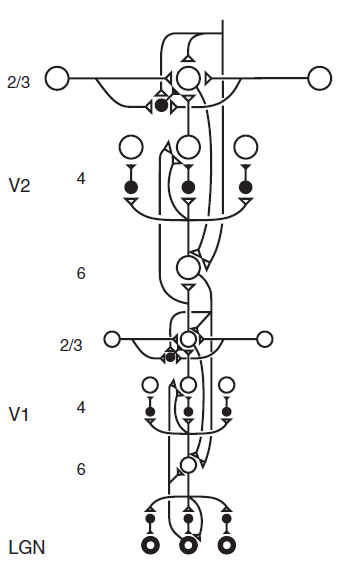
\includegraphics[width=0.3\textwidth]{canonicalcircuit}
	\end{center}
  \caption{Canonical cortical circuit}
  \label{fig:cortical_circuit}
\end{wrapfigure}
There is increasing concurrence that biological vision systems adopt a hierarchical and complementary computing paradigm \cite{Grossberg2000a}\cite{Grossberg2007} to achieve high level vision. The ventral and the dorsal streams of the visual cortex compute complementary properties. The ventral stream also called the \textit{what stream} is responsible for visual recognition and it comprises of cortical areas V1-V2-V4-IT-PMC\cite{MarkF.Bear1996}. From V1 to IT, increased receptive field sizes and complexity of the incoming stimulus has been observed. Experiments\cite{Tanak1996} show the presence of IT cells which respond selectively to objects. These cells are hypothesized as being invariant to transformations of objects. With experiments done on the cat's striate cortex by Hubel and Weisel \cite{D.H.Hubel1977}revealing several properties of the simple and complex cells of the Primary visual cortex and several following anatomical studies, the visual cortex is one of the most extensively studied areas of the brain. The huge amount of behavioral, pyscho-physical and anatomical data collected by studies performed on the Visual Cortex gives rise to a massive hypothesis space. Many computational models built on the broad principles of a set of popular and narrowed hypothesis space have shown state of the art performance on all the bench mark data sets. These models help further narrowing the hypothesis space and are used in complement to anatomical studies to understand the underlying mechanisms of vision. Grossberg 2007\cite{Grossberg2007} presents the LAMINART model which gives a comprehensive overview of the basic principles of cortical computing. A brief summary of two of the principles relevant to this paper presented in LAMINART, Hierarchical feedforward computing and feedback computing(attention modeling)\cite{Grossberg2007} is presented below . Figure~\ref{fig:cortical_circuit} shows the structure of the canonical cortical circuit(which repeats itself across all the cortical layers\cite{Grossberg2007}). Each cortical area can be broadly segregated into 6 hierarchical layers. \\

\textit{Feedforward Computing: }Layers 2/3 of the lower cortical areas with smaller receptive fields pool together to provide bottom up activation into layer 4 of the next layer up the hierarchy with larger receptive fields both directly and indirectly through layer 6 - 4 route as shown in Figure~\ref{fig:feedforward}. \begin{wrapfigure}{r}{0.2\textwidth} 
	\begin{centering}
		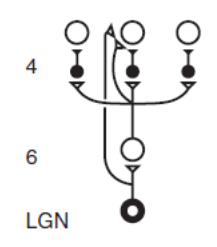
\includegraphics[width=0.2\textwidth]{feedforward}
	\end{centering}
  \caption{Feedforward}
  \label{fig:feedforward}
  \begin{centering}
		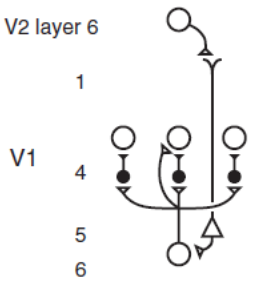
\includegraphics[width=0.2\textwidth]{feedback}
	\end{centering}
  \caption{Feedback}
  \label{fig:feedback}
\end{wrapfigure}The input connections through the layer 6 -4 route provide inhibitory activation to the surrounding neurons increasing sparseness while providing both inhibitory and excitatory activation to the neuron to which a direct connection is made providing a modulatory effect and resulting in  gain control and contrast divisive normalization. This form of processing in the visual cortex is believed to be used by the visual cortex in recognition of simple and unambiguous scenes in which processing speed is very high\cite{SimonThorpe1996}.\\ 

\textit{Feedback Computing: }Higher cortical areas provide both excitatory and inhibitory activation to layer 4 through the same layer 6-4 route as in feed forward processing as shown in Figure~\ref{fig:feedback}. This form of activation is said to be used in recognizing objects in a visual clutter where processing time is comparatively much higher than in unambiguous object recognition. Increased competition in the network decreases all the cell activities and the connections from higher cortical areas which share the same connections as in feed forward processing selectively increase the cell activities while inhibiting the activities of the surrounding cells. The network behaves like a dynamical system which rapidly increases the contrast between the winner(determined by feedback) and the rest of the neurons in the competition until the system reaches an attractor, the cell activity of the winner neuron crosses a threshold and provides activation to higher cortical areas. These properties are selectively adopted in several biologically inspired artificial vision models\cite{Fukushim1980}\cite{JimMutch2008}\cite{MarkusLessmann2014}\cite{NicolasPinto2008}\cite{ThomasSerre2007}\cite{XiaolinHu2014} with varying parameters that model the different features mentioned above.
\section{Problem of Invariant Object Recognition}
\label{sec:objectrecognition}
The major hurdle in building artificial vision systems has been to achieve recognitions invariant to translation, rotation, scaling and minor distortions and to build efficient 3D object representations.The problem of invariance in object recognition forms the core of the problem of object recognition\cite{JamesJ.DiCarlo2007}. Images of any real world object can occur in nearly an infinite number of forms in terms of position, scale, orientation, illumination, geometrical deformations etc\cite{NicolasPinto2008}. Leibo et al.\cite{rohtua} define two forms of invariance in object recognition, generic invariance which corresponds to invariance to transformations of a single object and Class specific invariance which corresponds to constructing a system which can read out class identities of objects belonging to a particular class. This paper talks only about generic invariance as defined above\cite{rohtua} and invariance to any other properties is beyond the scope of this paper. Experiments show that the ventral stream gains invariance slowly from V1 to IT. IT populations are known to show generic invariance while demonstrating selectivity to object identities\cite{HungCP2005}. When different transformations of objects are presented to a visual recognition system, the system should essentially be able to define a decision function that can separate the images belonging to transformations of the same object from images belonging to transformations of different objects\cite{AshbyFG1988} . The learning of this decision function can be supervised, unsupervised or a semi supervised manner. To enable this the architecture transforms the representation of the input image. At each level, a combination of dimensionality reduction and dimensionality explosion is observed\cite{JamesJ.DiCarlo2007}. This problem can be seen as the problem of untangling object manifolds\cite{JamesJ.DiCarlo2007}(each manifold corresponding to different transformations of an object plotted together in the representation space \cite{Edelm1999}) in stages such that each stage learns the function which, when applied on its input untangles local distortions. A classifier which takes the output of the highest layer in the hierarchy produces a discriminant function. A standard model of the visual cortex used in computational models for object recognition consist of a hierarchy of layers of S and C cells corresponding to the simple and complex cells\cite{D.H.Hubel1977} found in the visual cortex. The simple cells show selectivity to their optimal stimulus and the complex cells which have greater receptive fields pool over the simple cells and achieve invariance to local transformations. The weights of the connections across the layers, number of layers in the hierarchy and input representation are some of the parameters that affect the efficiency of recognition in the visual system. In the next section, we discuss models for object recognition inspired by the Visual cortex.
\section{Cortically inspired Vision systems}
\label{sec:corticalmodels}
Many biologically inspired visual recognition models have their foundations in the Neocognitron model.\cite{Fukushim1980}. This paper briefly discusses the following models. SMF model (Serre et al.,) \cite{ThomasSerre2007}, a revised model of HMAX\cite{MaximilianRiesenhuber1999}, SLF model (Mutch et al.,) \cite{JimMutch2008}, Sparsity Regularized HMAX model (Xiaolin et al.,) \cite{XiaolinHu2014}, V1 like model (Pinto et al.,)\cite{NicolasPinto2008} and Lessmann et al., \cite{MarkusLessmann2014}

\textit{SMF Model: }The architecture of this system consists of 4 layers (S1,C1,S2,C2) arranged in a hierarchical structure. S1 cells are modeled after the simple cells of the primary visual cortex whose receptive field is mathematically described\cite{JPJones1987} by a Gabor Function(see equation below)\cite{Gabor1946}. A Gabor function is given by a convolution of a sinusoidal with a Gaussian and hence it behaves like a localized cosine transform detecting the spatial frequency in the neighborhood. 
\begin{equation}\label{eq:Gabor}
F(x,y) = \exp(-\frac{x_0^2 + \gamma^2y_0^2}{2\sigma^2})*\cos(\frac{2\Pi}{\lambda}x_0), \quad where 
\end{equation}
\begin{equation}\label{eq:Gabor_or}
x_0 = x\cos(\theta)+y\sin(\theta) \quad and \quad y_0 = -x\sin(\theta) + y\cos(\theta))
\end{equation}
$\theta $ determines the preferred orientation of the Gabor filter and SMF model uses 4 orientations $(0^0,45^0,90^0,135^0)$. The other parameters of Gabor filters are determined based on experimental data generated by the behavior of V1 simple cells\cite{ThomasSerre2004}. 16 different scales are used in the model to induce invariance to scale. C1 cells with larger receptive fields(depending on the size of the scale band)\cite{ThomasSerre2007} pool over scales(2) of S1 cells to achieve slight position and scale invariance while maintaining orientation selectivity by pooling over S1 cells with the same preferred orientation. A Max operation is used on the pool of efferent S1 cells to determine the output of C1 cells. S2 units compute the distance(Gaussian of the Euclidean distance) from their inputs to stored prototypes for all scales. The prototypes are stored in the same format as the output of C1 during the learning phase. C2 cells pool over all scales and positions using a MAX operation testing the maximum distance between the features of the image and the prototype vector, i.e essentially C2 units check for the presence of a prototype vector anywhere in the image in any scale. Finally a SVM is applied on the output of C2 units to obtain the decision function. \\

\textit{SLF Model(Mutch et al.,):} This model\cite{JimMutch2008} is based on the SMF model described above\cite{ThomasSerre2007}. In this model, an image pyramid(of scales) is created and is used as input to the network. S1 filters are normalized and an additional normalizing parameter is included in S2 to modulate the effect of varying patch sizes in feature template matching. Apart from these fine tuning changes, a few other changes are made to the model. \textit{Increased sparseness:} As we recall from the SMF model, S2 performs a feature template matching by calculating the distance between each feature and a prototype across all orientations for all scales thus essentially using the combination of distances between the prototype and each of the orientations. In the SLF model, sparseness in increased for inputs to S2 by considering only the distance between the prototype and the strongest orientation for each position. However as the model now computes the presence of an orientation like an on or off function, more number of orientations(12) are used to maintain the accuracy. Additionally to inhibit the output responses of S1 and C1 cells, weakly active neurons are suppressed by defining a global parameter which determines the fraction of cells that are inhibited. Sparsity is further improved at the classification stage by selecting only the features that are highly weighted. \textit{Partial retention of position/scale information:} Unlike the SMF model which achieves complete position and scale invariance by applying a MAX operation over all positions and scales, the SLF model only pools over a large receptive field(smaller than the size of the image) both in position and scale.\\

\textit{Sparse HMAX}\cite{XiaolinHu2014}: This model modifies HMAX\cite{MaximilianRiesenhuber1999} mainly by learning the filters of all S layers using sparse coding methods (Independent Component Analysis\cite{AapoHyvaerinen2009} and Standard sparse coding\cite{XiaolinHu2014}). The model allows for layers at levels higher up the hierarchy. A few other fine tuning changes are made to the model which are not relevant to the evaluation performed in this paper and are hence not mentioned.\\

\textit{V1 like Model}\cite{NicolasPinto2008}: (Pinto et al., 2008) designed a baseline model(referred to as a Neuroscience null model in \cite{NicolasPinto2008}) based on the receptive fields of the simple cells found in V1. In the model, normalized images are convolved with normalized Gabor filters(eq \ref{eq:Gabor}) and with 16 different orientations(eq \ref{eq:Gabor_or}) and 6 spatial frequencies(which can model the receptive fields of V1 simple cells\citep{BrunoA.Olshausen1996}) after first applying a local normalizing filter to the input image. This local normalizing step is intended to model the local divisive normalization found in V1 simple cells\cite{Heeger1992}. The filtered images are subjected to thresholding and saturation and are further subjected to local divisive normalization.\\

\textit{Lessmann et al.,: } This model is similar to the Memory Prediction Framework\cite{Hawkins2004}, \cite{DileepGeorge2009}, \cite{George2008} which is based on the ideas of laminar computing, temporal sequence learning and attention modelling to achieve invariance in object recognition. The first primary difference between this model and the ones described above is the use of temporal sequences to learn invariance.\\

\textit{Basic features of the model: } 
\begin{itemize}
\item The computing architecture, similar to HMAX\cite{MaximilianRiesenhuber1999} and the other models summarized above takes a laminar form with several stages (3 or 4) with each stage consisting of two sublayers referred to as S and T layers in \cite{MarkusLessmann2014} corresponding to spatial neurons and temporal neurons respectively.
\item During the recognition stage, at the lowest level activation is computed through parquet graphs\cite{westphal-feat} which are Gabor jets\cite{Gabor1946} placed on a sampled grid  and the activation of all other neurons are computed as a hyperbolic tangent of the weighted sum of the afferent inputs converging onto that neuron\cite{MarkusLessmann2014} as given below. \begin{equation}
Act_i = \tanh\sum\limits_jW_{i,j}Act_j, 
\end{equation} 
where  $W_{i,j}$ are the weights between the neurons i and j learned during the learning phase. They encode a defined similarity between the input to the node and the prototypes stored at each layer.
\item For spatial neurons after computing the feedforward input, lateral inhibition is applied to the inputs by setting all but the K most active neurons to zero both to improve sparseness in feature representation and to prevent the system from running into over excitation.
\item Additionally the spatial neurons that remain active after applying the lateral inhibition receive feedback from the temporal neurons that have been active in the past T time steps(This information is recorded by storing the activities of all neurons into what is referred to as an activity stack\cite{MarkusLessmann2014}).
\item Inputs and activation of temporal neurons is the same as that of spatial neurons except that temporal neurons receive feedback only from the activities of spatial neurons in the higher layer for the last presented image and not the last T images. 
\item During learning a Codebook of features is learned at each level of spatial neurons first by defining an empty codebook and a similarity function. If the current extracted input features are within the pre defined threshold of the similarity function, the codebook remains unchanged else the codebook is updated with the input features of the current image. 
\item To form the temporal groups, an adjacency matrix is created with the element (i,j) of the matrix representing, for every node, the probability that the neurons at locations i and j were active at some time in the past T time steps. Spectral clustering\cite{UlrikevonLuxburg2004} is then used to form temporal groups which serve as inputs to the spatial nodes in the next layer. 
\item Thus essentially, S layer detects the spatial patterns in the input signal and the T layer determines the temporal group of the input signal with an associated probability. 
\item Also, Each node\cite{MarkusLessmann2014} of the S layer at each stage is connected to one node of the T layer in the same stage and a group of nodes (usually 9) make an afferent convergence into one node in the S layer of the subsequent higher stage in the hierarchy. 
\item Training is not done simultaneously for all layers but can only be performed layer by layer.
\item The system has to be trained from sequences that represent images undergoing a particular transformation in order for the network to develop invariance to that transformation. 
\item The Activity stack is emptied after presenting each object category to prevent learning associations between different object categories.

\end{itemize} 	
Technical details not relevant to the discussion in this paper are excluded and can be referred to in \cite{MarkusLessmann2014}

\section{Analysis and Discussion}
\label{sec:Eval}
Cortical computing for object recognition is indeed highly complex and the models summarized above belong to a family of hierarchical models which attempt to model certain aspects of the principles of cortical computing summarized in section \ref{sec:Cortical Computing}. There are various questions that need to be answered in order to integrate these models into an optimally unifying architecture. Some of the questions that need to be answered are listed below. 
\begin{itemize}
\item Which principles of cortical computing are relevant to solving the problem of invariant object recognition? 
\item Which computing architecture is better suited to learn invariance in object recognition? 
\item Which mathematical models can approximate the processing of the cortex? 
\item Which mathematical models optimize the behavior of the neurons?
\item What is the effect of the parameters like the number of neurons, number of selected features and the parameters used in the hardcoded Gabor filters? 
\item Is it efficient to use hard coded mathematical models that estimate the behavior of cortical elements or is it more efficient to learn the properties by training on a good statistical sample of images?
\item What is a good statistical sample that can efficiently represent the variability of the object in a real world scenario?
\end{itemize}
The list of questions that can be answered is quite vast and answering all of them is beyond the scope of this paper. Hence this paper focuses on answering a small subset of these questions. 
\subsection{Feedforward Computing vs Feedback Computing}

All the models belonging to the class of hierarchical models adopt a feedforward computing mode. Experimental data shows that IT populations of neurons respond to visual stimuli within 100ms\cite{ChouP.Hung.GabrielKreiman2005} with a high degree of accuracy. Such rapid recognition rates of processing the signal through what is known to be an extremely complex network seems to indicate that feedforward processing is mainly used in visual object recognition\cite{ThomasSerre2007a}. The SMF model, SLF model and SPARSE HMAX model, convolutional networks\cite{K.Kavukcuoglu2009},\cite{Krizhevsky2012} belong to the class of such feedforward models. The authors of these class of feedforward models recognize the limitations of such a feedforward architecture. 

Anatomical studies like \cite{BoyapatiJ1984},\cite{Montero1991} show that the number of feedback connections in both intra and inter cortical areas far surpass the number of feedforward connections between them. This causes the existence of a different class of models hypothesizing that feedback probably plays an important role in cortical processing\cite{Macknik2007}. \cite{MarkusLessmann2014},\cite{DileepGeorge2009} are models that belong to this class.\\
The feedforward Architectures discussed above can not be categorized as strictly feedforward models as the nonlinearities in the networks such as local divisive normalization or the max operation would need to utilize local feedback connections to be implemented in a strictly neural architecture. This does not contradict the anatomical and physiological evidence of extremely rapid recognition in the first 150ms of the presentation of the stimuli. If any evidence is presented in the future that back projections are utilized in visual recognition in the first 150ms, then these architectures could be restructured to incorporate them. Back projections could be utilized to, for instance, perform segmentation or selective computation of neuronal activities in the lower layers depending on the object category. Lessmann et al.,\cite{MarkusLessmann2014} utilizes feedback from higher cortical layers as well as within the same cortical area to utilize principles of  spatial continuity and temporal trace learning to achieve invariance to many transformations. However physiological data shows that synaptic plasticity(Long term potentiation or long term depression) depends on calcium dynamics according to which calcium levels at synaptic sites encode a trace of neural activity. This evidence points towards a different role for the back projections in the neural circuitry which is yet to be completely determined. 

 To sum up, feedforward processing has the advantages of being simple and fast but the design principles do not deal with ambiguity in visual scenes, which is an element of real world scenes.Visual attention, focusing and selective learning are hypothesized as utilities of back projections in the neural circuitry. Feedback connections that modulate the responses of the lower layers could be an effective tool to eliminate the competition between competing neurons in the presence of an ambiguous stimulus. The feedforward models could be integrated into a visual system with greater computational capability which include other principles observed in cortical computing such as attention modeling or perceptual grouping\cite{Grossberg2007}. Certain non HMAX like models have attempted to incorporate top down inference in the models to resolve ambiguities by generating predictions.\cite{HonglakLee2009} uses undirected Deep belief networks(with stacked RBM's) and probabilistic max pooling\cite{HonglakLee2009} to achieve translation invariance and recognition in ambiguous as well as occluded scenarios. In this paper we try to address various parameters of the feedforward mode(not to be misinterpreted as a strictly feedfoward neural architecture) of computing that affect the performance of recognition.
\subsection{Statistics of Natural Images}
\label{Subsec:NatImStat}
Strong evidence\cite{BrunoA.Olshausen1996} and several other theories have strongly supported the claim that the visual system(all cortical areas) adapts itself to the statistics of the inputs that it processes. Which means that the change in representation is optimized to suit the statistics of natural images and only focuses on those aspects of data which are essential for further analysis\cite{AapoHyvaerinen2009}. This implies that the processing of the visual system is influenced both by genetic information and visual experience. In light of this theory it would be a good idea to look at the statistics of the natural images to identify useful representations. If we look at a statistical distribution of natural images the distribution is highly skewed(non normal) i.e, there is a high amount of redundancy in the natural images\cite{AapoHyvaerinen2009}. This fact has led the vision systems to draw inspiration from Information theory(Image compression). Each natural image consists of much higher amount information than is required to represent it. The objective of the visual system is then to eliminate the redundancy and to represent the image in least number of bits(features). Apart from the number of bits there are also other criterion such as ease of processing. This adds additional constraints to the transformation of representation. The concepts of sparseness of representation, dimensionality reduction, unsupervised learning stem from this approach and this paper discusses each of the aspect in some detail.  The main objective however seems to be that the prime role of the cortical units is to reduce the statistical dependencies between the basis functions representing the image. We will look at why this is essential in the next section. 
\subsection{Dimensionality of Input - Output spaces}
\label{Subsec:Dimen}
The principle of HMAX like architectures can be described in the perspective of untangling object manifolds\cite{JamesJ.DiCarlo2007}. The objective is to uncover the underlying low dimensional object manifolds which lie in a high dimensional feature space and at the same time untangle the manifolds such that a simple hyperplane(a linear classifier) could separate the classes. This view incorporates two basic ideas of dimensionality explosion and dimensionality reduction. Dimensionality reduction is achieved by mapping similar(determined by a pre defined similarity) images in the input space onto a low dimensional manifold thus extracting the underlying manifolds. This step needs to be followed by change in representation of the inputs by projecting the manifolds onto a much higher dimensional space(overcompleteness) to establish statistical independence between the inputs to achieve untangling. In HMAX like architectures a hierarchical approach to untangling is incorporated where each layer untangles local subspaces\cite{JamesJ.DiCarlo2007}. 

This can be visualized in the figure \ref{fig:Untangle}. This view supports the view of complementary cortical processing where each cortical area or even each sub cortical area could be viewed as independent processing units computing properties(untangling local subspace manifolds) thus providing an abstraction to enable further processing.  
\begin{figure}[h]
\begin{center}
\includegraphics[scale=0.3]{manifolds}
\end{center}
\caption{Untangling object manifolds \cite{JamesJ.DiCarlo2007} }
\label{fig:Untangle}
\end{figure}
Several dimensionality reduction techniques exist in literature. Principle Component Analysis(PCA), Local Linear Embedding(LLE), Dimensionality reduction by learning an invariant mapping(DrLIM) and several other linear and non linear dimensionality reduction techniques map similar inputs in a high dimensional input space to neighboring points in a low dimensional manifold. These methods however can not be useful by themselves as they map all the training samples to the same low dimensional manifold which does not conform to the view under our consideration. These techniques could however be employed with slight modifications along with additional constraints of sparsity of representation to achieve the required change in representation. For instance sparse coding unlike many other dimensionality reduction techniques can be used to learn overcomplete basis of representation. These techniques identify the basis vectors used to represent the input data. The goal is to identify the set of basis vectors which can represent the input space with maximal efficiency. Dimensionality reduction techniques identify low dimensional structures in a high dimensional input space. 
\subsection{Feature extraction}
\label{Subsec: Feature}
The class of models this paper focuses on contains linear and non linear transformations of the input images in several stages. Each stage usually consists of two different kinds of layers and sub processing stages. The first layer corresponds to a linear filter and the second stage corresponds to a non linear filter. The processing in the visual system can be viewed as a trade off between selectivity and invariance. The linear filters show selectivity to their desired input configurations and the non linear pooling layer achieves invariance by pooling over the cells in the lower layers. In this subsection, we discuss various properties of the linear filtering layer.

\textbf{Extraction of low level features:}
Filters that extract these features in each of the stages can either be learned in a supervised/unsupervised/semi-supervised manner or they can be built based on previous knowledge of the statistics of the images that will be encountered by the network. Biologically inspired models \cite{Fukushim1980},\cite{JimMutch2008},\cite{MaximilianRiesenhuber1999},\cite{NicolasPinto2008},\cite{ThomasSerre2007},\cite{MarkusLessmann2014},\cite{XiaolinHu2014} popularly use Gabor filters\cite{Gabor1946} for learning low level features of images which have been proven to be good mathematical descriptors of receptive fields of the simple cells in V1\cite{JPJones1987}. Other models\cite{K.Kavukcuoglu2009} and single stage feature extraction systems use feature descriptors like Scale Invariant Feature Transform (SIFT)\cite{Lowe2004}, Histogram of Gradients(HOG), Geometric Blur\cite{BergA.C2001},\cite{HaoZhang2006} \cite{NavneetDalal2005} to extract low level features. Several evaluation studies\cite{Mikolajczyk2005} compare low level feature descriptors and there seems to be increasing concurrence that SIFT\cite{Lowe2004} descriptors with some modifications are the best performing feature descriptors for object recognition. However these studies do not evaluate\cite{NicolasPinto2011} the performance of these feature descriptors in tackling the so called invariance problem\cite{NicolasPinto2008}. A screening approach similar to \cite{NicolasPinto2009} which test the effect of different feature descriptors while maintaining all the other parameters on different datasets can determine the ideal feature descriptor to be used in the first stage of the feedforward models. Other models\cite{K.Kavukcuoglu2009} learn these low level features in an unsupervised manner or supervised manner. 

The neocortex looks remarkably similar across different processing systems which led to the hypothesis that a fundamental principle of cortical computing underlies all the sensory processing systems\cite{VB1997} of the brain and each processing system develops its abilities by learning through statistical properties of the stimuli fed into that processing unit. This claim is in conformity with the hypothesis from information theory. Supplementing this claim, Oshlausen et al.,\cite{BrunoA.Olshausen1996} show that unsupervised learning using sparse coding(discussed later in the paper) strategy when trained on natural images generates filters which behave like the receptive fields of simple cells in V1(Gabor Filters)\cite{JPJones1987},\cite{Gabor1946}. Using Gabor filters to extract  features in the low level stages are effective due to their sparseness(dependent on the parameters) and hence can effectively reduce the statistical dependencies\cite{BrunoA.Olshausen1996} between the input images which is essential to untangle object manifolds\cite{JamesJ.DiCarlo2007}. However Gabor filters can not be considered to be suited for any general input image as the features can be learned depending on the statistics of the input signals. The next question in this approach would be which supervised or unsupervised learning method can be used to learn the features. Sparse HMAX\citep{XiaolinHu2014} uses standard sparse coding which is a variant of the independent component analysis with an additional sparsity constraint to learn the low level features which gives rise to Gabor wavelets. The idea of sparse coding is to decompose the input space into a large number of basis functions with additional constraint that the number of basis functions used to represent each input signal is very low. However, the choice of sparse coding to learn the features is rather ad hoc apart from good intuitive appeal. For instance \cite{HonglakLee2006} achieves sparse coding by solving a L1-regularized least squares problem and L2-constrained least
squares problem. A theoretical approach to obtaining maximally independent(statistical independence) and sparse low level feature components would be an interesting approach to solve this problem. 

\textbf{Mid level features}\\
Although the mathematical behavior of V1 simple cells is well described by Gabor filters, the behavior of the cortical cells in the remaining layers of hierarchy is not well known and no such mathematical descriptor exists that describes the behavior of these cells. Hence these properties need to be learned according to the same principle as we discussed above. SPARSE HMAX\cite{XiaolinHu2014} attempts to learn these features for all stages using Independent Component Analysis and Standard Sparse Coding\cite{XiaolinHu2014}. It shows significant improvement in performance over HMAX\cite{MaximilianRiesenhuber1999}. 

\cite{KevinJarret2009} shows that for a generic set of images where the image statistics are not previously known, learning the filters rather than applying random filters(which may have shown good performance on images which do not follow the same statistical properties) considerably improves the performance of these systems on visual recognition. \cite{KevinJarret2009} also shows that feature extraction in two stages are better than one stage feature extraction. Even though the analysis in the paper was based on empirical evidence, the architectures under consideration in this paper are biologically inspired and from the discussion above we know that the output of V1 passes through  a series of other cortical areas before it reaches IT, where object recognition is known to be taking place.
The features extracted in the first stage are passed through a coding stage and a pooling stage to become mid level features. All the HMAX like architectures described above \cite{Fukushim1980},\cite{JimMutch2008},\cite{MaximilianRiesenhuber1999},\cite{ThomasSerre2007} use randomly selected patches of features and compare them to templates stored during the learning phase. This method of choosing mid level features is sub optimal and this is recognized by \cite{XiaolinHu2014}. Sparse HMAX learns the mid level features using standard sparse coding. \cite{MarkusLessmann2014} learns the mid level features using vector quantization and clustering the features with spectral clustering. 

Ideal mid level features should have the same properties as the low level features such as sparseness, compact low dimensional representation of similar objects on a low dimensional manifold, i.e they should have properties that reduce the statistical dependencies between input signals.HMAX like architectures and V1 like model\cite{NicolasPinto2008} use non linearities namely contrast divisive normalization and horizontal inhibition to increase sparseness both of which reduce statistical dependencies. We will discuss these non linearities in further detail in the next sub section. \cite{Y-LanBoureau2010} shows that learning the mid level features using sparse coding is better than using hard vector quantization or soft vector quantization in terms of enhanced performance. However as we discussed in the context of sparse coding, other methods of unsupervised learning for both mid level features as well as low level features have not been sufficiently explored yet. 

Techniques such as spatial pyramid matching have been proven to be very efficient in identifying mid level features but biologically inspired HMAX like architectures refrain from deviating from the hypothesis of untangling object manifolds and this approach works in complement with computational neuroscience research in identifying the underlying mechanisms of visual recognition. Hence we do not discuss these methods for learning mid level features in this paper.

\textbf{Computing High level features}
By high level features we mean the output of the highest layer of the neural architecture. Bag of words model works by identifying the frequency of all the features in the input image. This method loses all the spatial information but it has been proven to be very successful in HMAX like architectures. This is due to the fact that each object representation is quite sparse and uses very few basis functions to represent the image. It has to be noted that this approach is applicable to natural scenes but can not be extended to any general image. However complete loss of spatial information is not a desirable property as some amount of spatial connectivity might be essential in identifying target objects. Also, IT cells in the visual cortex are not completely invariant to translation. They retain certain amount of spatial information. \cite{JimMutch2008} adopts this view and retains some amount of spatial information. \cite{XiaolinHu2014} uses spatial pyramid matching to achieve the same. Spatial pyramid matching has been proven to be very effective in enhancing the performance of invariant object recognition systems.
\subsection{Non-linearity}
\label{Subsec: Nonlinear} Feature extraction stages involve more than simple feature descriptors. Hierarchical models use non linear functions such as application of a non linear activation function, local divisive normalization/local contrast normalization, lateral inhibition, rectification, pooling etc. As the models attempt to untangle manifolds, linear functions are not sufficient to perform the task. Any set of linear basis functions, even if they are designed to maximize statistical independence and hence to eliminate second order dependencies still show higher order dependencies\cite{EeroP.Simoncelli1999} which violates the efficient coding hypothesis. Hence non linear functions need to be used to reduce the statistical dependencies between image representations\cite{Bethge2006},. Methods such as local divisive normalization, lateral inhibition, pooling are biologically inspired as they are found in cortical circuitry of the neocortex. Biologically inspired models use these non linearities and an improved performance has been recorded after applying some of the non linearities as it was expected.

\textbf{Non linear activation function: }All well known and accepted models of neurons like the Hodgkin Huxley Model\cite{Hodgkin1952} and even the simplest models of a neuron like the perceptron\cite{Rosenblatt1957} use thresholding as it is observed in the generation of Action potentials in the neurons. Thresholding is usually modeled by sigmoidal or hyperbolic tangent functions. HMAX inspired models do not explicitly use thresholding as they use a set of prototype features to compare with by defining a similarity function usually using functions with higher degree of kurtosis.

\textbf{Contrast divisive normalization: }Responses of V1 cells can not be completely determined by linear processes. It has been shown that contrast divisive normalization explains some of the non linear behavior exhibited by the neurons\cite{Bonds1989}. This includes taking the absolute value of the output signal(rectification) and dividing it with a weighted sum of absolute values of responses of all the other neurons. As we have discussed above, this mechanism can not be realized by a strictly neural architecture and local feedback connections which is also demonstrated in section \ref{sec:Cortical Computing}. \cite{Bonds1989} also shows that applying divisive normalization to the output of pairwise, maximally statistically  independent cells can be eliminated by applying divisive normalization. To maximize the effect of this non linearity, the parameters involved need to be optimized which are the weights and the bias term added to the denominator of the function.\cite{RobertoValerio2003} exploit knowledge on statistics of natural images according to which conditional histograms of coefficients of the basis functions of nearby cells approximately fit a Gaussian distribution\cite{SchwartzO2001} and create a measure of statistical independence to arrive at optimal values for parameters. This could be utilized to minimize higher order statistical dependencies. \cite{KevinJarret2009} shows that even systems that use random filters without any sort of learning show considerably good performance as long as they included rectification and divisive normalization. Also,\cite{EeroP.Simoncelli1999} shows that the optimal parameters of the function adapted to the statistics of natural images give rise to functions which explain the suppression of responses to stimuli presented outside the classical receptive fields of neurons in the primary visual cortex. This further strengthens our view of optimal coding hypothesis and the view that cortical processing adapts itself to the statistics of the signals encountered by the system.  

Apart from rectification and divisive normalization, \cite{JimMutch2008},\cite{MarkusLessmann2014},\cite{ThomasSerre2007} also use lateral inhibition as a non linearity to further sparsify the feature representation, the effects of which have been discussed above. 

\textbf{Pooling}
Pooling is a crucial property of cortical processing to achieve invariance. As discussed in section \ref{sec:Cortical Computing}, receptive field sizes increase as one moves up the cortical processing stages of hierarchy thus achieving higher levels of translation invariance. HMAX like architectures, convolutional neural networks and other biologically inspired models of invariant object recognition involve pooling and subsampling. The objective is to retain relevant information while sacrificing certain amount of selectivity. Pooling of the high level features has already been discussed above(Ref: Subsection \ref{Subsec: Feature}). We now discuss pooling strategies of the intermediate layers of hierarchy.
\begin{wrapfigure}{r}{0.5\textwidth} 
	\begin{centering}
		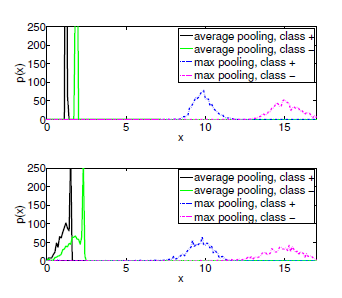
\includegraphics[width=0.5\textwidth]{pooling}
		\caption{Pooling}
	\end{centering}
  \label{fig:pooling}
\end{wrapfigure}
Most common pooling techniques used to achieve invariance to translation and scale are average pooling or max pooling. There is strong empirical evidence in favor of max pooling over average pooling\cite{Y-LanBoureau2010} and most latest research(relevant) in has adopted max pooling as it consistently showed higher performance rates. However the reasons that underlie this increased performance can not be explained through empirical evidence. Also, the limitations to using Max poling over average pooling also can not be explained through empirical analysis. \cite{Y-LanBoureau2010a} performs theoretical analysis on a 2 class problem by analyzing the separability of conditional distributions of the feature representations given the class. This analysis can be extended to a multi class problem by just increasing the dimensionality of input space and the feature space. In the analysis, conditional distribution of image patches are modeled as a mixture of the distribution of the foreground and the distribution of the background(clutter). The clutter patches are present in both the classes as well as in varying amounts across the images.

The analysis of this model\cite{Y-LanBoureau2010a} shows that if the size of the pooling window is large then average pooling is robust to foreground variability where as max pooling does not show the same robustness. If the variance of either the clutter or the foreground is high then the average of the features causes the representations to spread increasing the amount of overlap\cite{Y-LanBoureau2010a} and thus reducing the separability of classes. In contrast max pooling can be robust to increased clutter if it is associated with a low mean. This is illustrated in the figure \ref{fig:pooling}. The results of the theoretical analysis also indicates that Max pooling shows higher performance efficiency over average pooling when the representation of the features is sparse. 

To sum up pooling strategy works best with max pooling over small pooling windows. If the mean of the distributions is low which is true after applying divisive normalization and the representation is sparse which is also true in the architectures we considered in this paper max pooling over small window sizes(the optimal size of the window should however be identified) would yield maximal efficiency of performance. 

Now that this is established, we look at the pooling strategy from a different point of view. Even with small window sizes with or with out overlap, max pooling pools features which can be highly dissimilar which may cause losing crucial and non redundant information regarding the image. The distribution of features could be highly distorted. This problem can be solved by using techniques similar to spatial pyramid matching. \cite{MarkusLessmann2014} defines a similarity between the spatial features as well as temporal groups and clusters them using spectral clustering. \cite{Y-LanBoureau2011} also demonstrates that local pooling in configuration space boosts performance. Performance in HMAX like architectures is likely to be enhanced by pooling in configuration space before the spatial pooling step. 
\subsection{Sparseness}
\label{Subsec:Sparsness}
There are different different kinds of sparseness that we have mentioned in the discussions above. Sparseness of features and sparseness of representation. It is essential to identify the differences between the two. For instance Gabor filters are considered to be sparse features but using gabor filters does not ensure sparsity of representations. The view of efficient coding hypothesis relies on developing good statistical generative models for natural images so that the prior probabilities essential for Bayesian inference can be obtained\cite{AapoHyvaerinen2009}. As we have established in the previous sections sparseness allows for a better statistical model that reduces redundancy thus improving what can be called the signal to noise ratio for optimal transmission. 

\subsection{Temporal vs spatial continuity}
\label{Subsec:TempSpat}
A popular hypothesis in the context of how the visual processing system learns invariance is that the cortex exploits the principles of temporal or spatial continuity(or both) to achieve invariance to translation, rotation, orientation, view point, perspective projections, illumination etc. The idea of temporal continuity is that images that fall on the retina which are close by in time are statistically far more probable to belong to the same object rather than two different objects. The idea of spatial continuity is that two different views of an object usually has sufficient overlap in terms of the neural activity which is encoded in the neural circuitry and hence the strengthened connections between the neurons lead to the same neural responses to two different views of the same object that have sufficient similarity(we do not define the similarity).

As the networks self organize to adapt to the statistics of the natural world and both temporal and spatial continuities are prominent features of the statistics of the visual stimuli, there is no reason for the network to not exploit both the features to learn invariance. However, if there is redundancy in terms of spatial and temporal continuity then to recreate such a network exploiting such redundancy could lead to higher computational efficiency which is also one of the prime goals of the visual processing system. 

\cite{MarkusLessmann2014} uses temporal continuity to achieve invariance to any chosen transformation. In this model, the spatial patterns are first grouped using a similarity(configuration pooling) and then the temporal groups are determined. The activities are stored in an activity stack. This acts as a temporal trace determining which temporal groups were active in an interval of time preceding the current time. If same neurons were active during the previous stages feedback sends excitatory signals indicating that the input images belong to possibly different views of the same object with high probability. Using temporal continuity to achieve invariance is a very efficient idea as it can create a unifying architecture that can create invariance to any kind of transformations that the network has been exposed to earlier during training. Many other recent deep learning architectures like slow feature analysis rely on temporal trace to achieve invariance to a wide variety of transformations. HMAX like architectures account for invariance to scale and position and depending on the pooling strategy some degree of invariance to rotation but they can not, in the current form, be scaled to integrate other forms of invariance. Temporal continuity is also very effective in creating 3D object representations. 

The idea of whether temporal or spatial continuity is adopted by the visual cortex has been very intriguing to the research community and several psychophysical experiments can be found in the literature supporting either of the views(or both). \cite{DavidDCox2005} show an interesting observation based on the idea that if temporal continuity were to be used by the brain to achieve invariance then the spatio temporal statistics of the images could be manipulated and the effects of which can be recorded. They induce predictable confusions in object identities by exposing the subjects to an altered world where objects changed identities during the transient blindness across saccades causing the subjects to associate different views of different objects that occurred closely in time to a single object.\cite{DavidDCox2005} further show that position invariance is not a property of the visual system but is an adaptation to the spatio temporal statistics of the natural world. 

Principles of spatial continuity on the other hand predict that in case of interleaved training(as described in the previous set up), invariance learning should not be impaired as the visual system still uses principles of spatial continuity to associate different views of the same object together.\cite{GavinPerry2008}. In this paper, we put forward some doubts that the setup of the experiment in \cite{GavinPerry2008} may not necessarily achieve what is referred to as interleaved training. The setup consists of presenting a test stimulus for 750ms, followed by a 500ms mask, followed by a blank screen for 250ms and then with a match or non match stimulus for 750ms. Our concern with this setup is that presentation of stimulus for 750ms may not necessarily be grouped as very short exposure as is claimed in the paper. This time scale is nearly 4-6 times the time scale needed for recognition in unambiguous images. Furthermore the participants were given practice sessions which enabled them to adjust to the time scales. Presentation of images for this time scale is sufficient for top down attention effects or even associations with existing objects in the memory thus leading to the same effects as predicted by spatial continuity.

However, as we mentioned above as spatial continuity and temporal continuity usually coexist, it is highly probable that the visual system exploits non redundant properties of both to achieve invariance.

\subsection{Miscellaneous Remarks}
This architecture of layer wise unsupervised learning bypasses problems such as local minima which are faced by many deep architectures. Many deep AI architectures struggle with the trade off between depth and viable learning rates.
This paper has not focused on a qualitative analysis based on empirical evidence of enhanced performance of different models when applied on benchmark data sets as we believe that the standard data sets may not sufficiently encapsulate the variability of real world images and hence the results of the tests are need to be passed through strict scrutiny before evaluating them which is beyond the scope of this paper. Our view is supported by \cite{NicolasPinto2008} where the authors create a V1 like model which by definition should not exhibit any invariance as a neuroscience null model which outperformed most state of the art visual recognition systems on CALTECH-101 which is considered one of the standard benchmark data sets for object recognition. 

\section{Conclusion}
\label{sec:concl}
Invariance, which is the crux of object recognition can be effectively achieved by taking inspiration from biological models. However the huge parameter space may often lead to misleading conclusions. The solution to this problem is to view each of the component in light of its theoretical guarantees and thereby constraining the parameter space. In HMAX like architectures we see that the main goal of the architectures is to achieve high degree of statistical independence so as to achieve efficient separability of object manifolds. All the components of the architecture are tuned to achieve this very goal and the optimal parameters for each component can be computed either through thorough theoretical analysis or a high throughput screening approach. In this paper we pave paths to construct what can be referred to as the optimal hierarchical architecture for object recognition.



%%%%%%%%%%%%%%%%%%%%%%%%%%%%%%%%%%%%%%
% hier werden - zum Ende des Textes - die bibliographischen Referenzen
% eingebunden
%
% Insbesondere stehen die eigentlichen Informationen in der Datei
% ``bib.bib''
%
\newpage
\bibliographystyle{plain}
\addcontentsline{toc}{chapter}{Bibliography}% Add to the TOC
\bibliography{Seminarwork}

\end{document}


